\documentclass{article}

\usepackage{graphicx}
\usepackage{hyperref}

\title{User Interface Parsing \\ \small{Progress Update}}
\author{Calvin Loncaric}
\date{June 1, 2015}

\begin{document}

\maketitle

\noindent Since the last update I have been working on layout generation from
parsed constraints. The system can now:
\begin{itemize}
\item convert parsed boxes and elements into constraints and
\item combine those constraints into a well-formed HTML document.
\end{itemize}

\noindent Regrettably, I was unable to get text recognition to an acceptable
level of accurracy (one of my goals from last time). This means that all box
distances and relationships are \emph{guessed} rather than being read from the
actual constraints written on the page. That said, the guessing is quite smart,
as you can see from Figure \ref{fig:screenshot}. My immediate next steps are:
\begin{itemize}
\item create a poster for the presentation on Wednesday,
\item test the tool on more complex cases, and
\item begin writing the final report.
\end{itemize}

\begin{figure}
    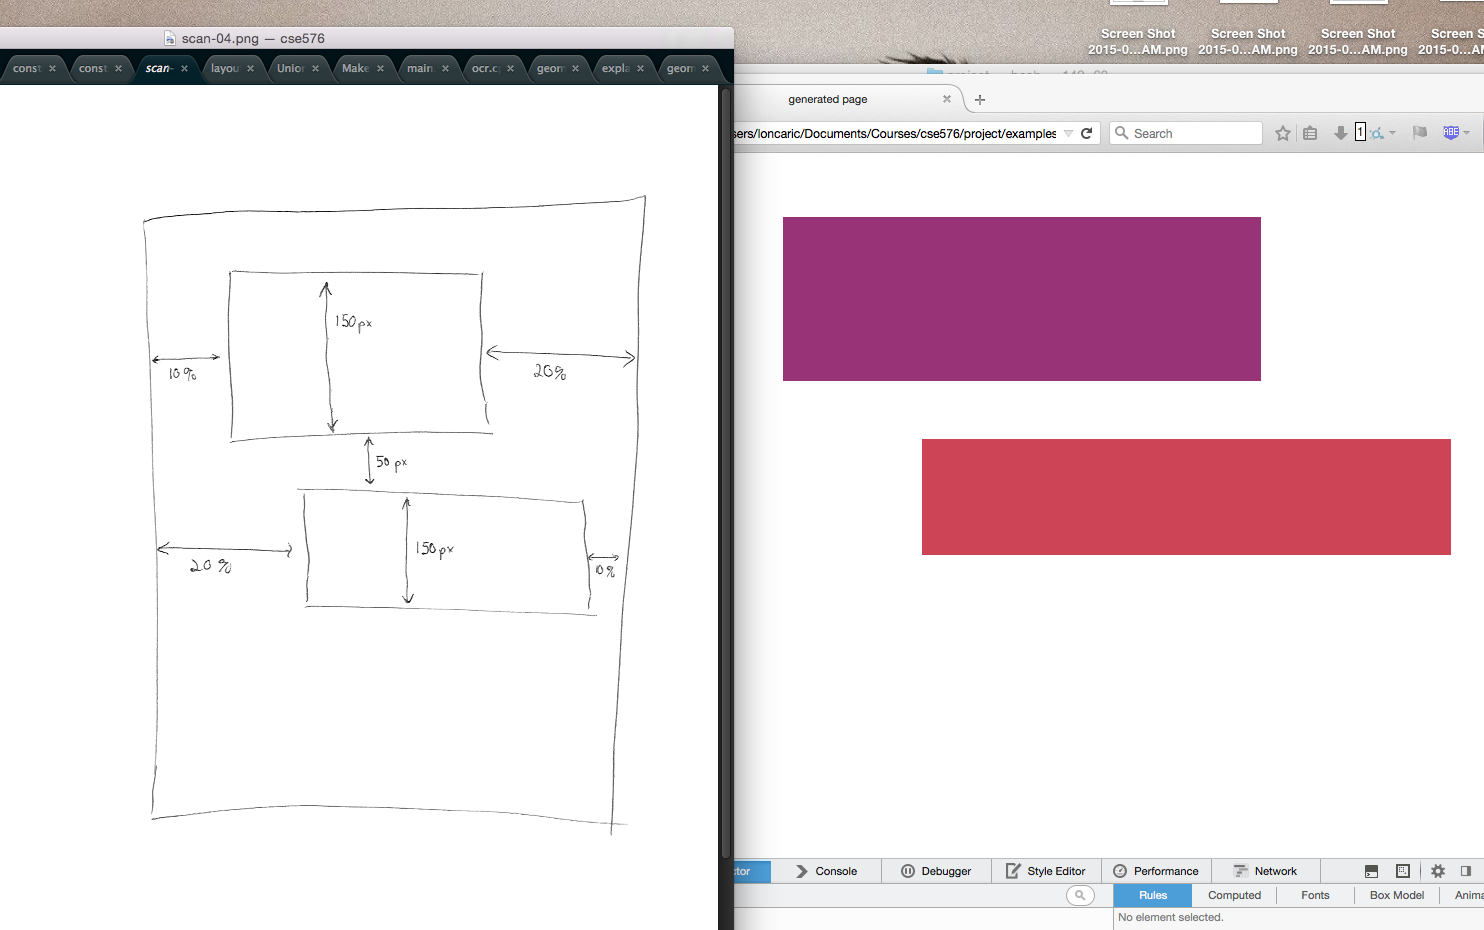
\includegraphics[width=\textwidth]{progress-2015-06-01-screenshot.png}
    \caption{Layout generation on one of the simpler test cases. The input
    image is shown on the left, and the inferred layout is shown on the right.
    The colors are generated randomly in order to distinguish boxes, but the
    HTML can (and should) be edited for style by hand.}
    \label{fig:screenshot}
\end{figure}

\end{document}
